\documentclass[a4paper]{article}
\usepackage[french]{babel}
\usepackage[utf8]{inputenc}
\usepackage[T1]{fontenc}
\usepackage{graphicx}   % pour les images
% \usepackage{svg}        % pour les svg (images vectoriel)
\usepackage{hyperref}   % pour les références
\usepackage{amssymb}    % pour les symboles de maths comme \mathbb{R}
\usepackage{mathtools}  % pour rajouter \text dans un environment math
\usepackage{subcaption} % pour les subfigures


\title{Rapport projet TLNL \\ Modèles de langages markoviens}
\author{Leader : Cléa Han | Follower : Adrien Zabban}
\date{5 novembre 2023}

\begin{document}

\maketitle

\section{Introduction}
 
Le projet consiste à programmer un modèle de langage markovien sous différentes modalités. À partir de ces modèles, nous 
allons en calculer les performances à l'aide de la métrique de la perplexité. Puis, nous allons implémenter le remplissage 
de textes à trous et la génération de texte. 

Pour approfondir notre étude, nous allons nous intéresser à l'évolution d'un modèle de langage markovien par rapport à la 
taille d'un corpus à la base de son apprentissage, afin d'en extraire sa courbe d'apprentissage. Puis, nous allons explorer 
la possibilité d'établir la paternité pour des textes de paroles de chansons et leurs auteurs. 

\section{Modèle Initial}

On s'intéresse ici à créer des modèles de langage markoviens : des n-grams. Ces modèles de langage sont en fait des probabilités 
conditionnelles de la forme $P(m_i|m_{i-n+1} \dots m_{i-1})$ où $n$ est l'ordre du modèle. Dans cette étude, nous nous 
restreignons à $n\in \{1, 2, 3\}$. Ces modèles seront entraînés et testés sur une base de données tirée d'\oe uvres d'Alexandre Dumas.

\subsection{Traitement des données}

On possède dans un premier temps un ensemble d'outils permettant de décomposer nos textes bruts en mots afin qu'ils puissent 
être traités dans le formalisme des modèles de langage markovien.
Cette opération de segmentation est appelée la tokenisation. Ensuite, nous coupons les textes en deux pour obtenir des textes d'entraînement, 
des textes de test. Cela nous permettra que nos $n$-grams apprennent sur les textes d'entraînement et de pouvoir mesurer leurs
performances sur les textes de test.

\subsection{Création des n-grams} 

À partir de fichiers textes tokenisés par les outils susmentionnés, nous allons calculer les probabilités n-grams d'un texte. Pour cela, on compte le nombre d'occurrences de toutes les séquences de longueur $n$ et $n-1$ du texte d'entraînement. Une fois que l'on 
connais l'occurrence de toutes les séquences, nous pouvons approximer la probabilité conditionnelle du mot $m_i$ sachant le contexte avec
l'équation~\ref{eq:ngram}.

\begin{equation}
    P(m_i|m_{i-n+1},\dots,m_{i-1}) \approx \frac{C(m_{i-n+1},\dots,m_{i-1},m_i)}{C(m_{i-n+1},\dots,m_{i-1})}
    \label{eq:ngram}
\end{equation}

où $m_i$ est le mot numéro $i$ du texte d'entraînement, $C(m_1,\dots,m_n)$ l'occurrence de la séquence $m_1,\dots,m_n$ dans le texte
d'entraînement\footnote{Avec la convention $C(\emptyset) = N$  le nombre de mots dans le texte.}. 

Cependant en procédant comme cela, le modèle ne pourra pas donner de probabilités sur des séquences qu'il n'a jamais vu,
faute d'avoir un dénominateur valant 0. Pour éviter cela, on utilise la formule de \textit{Laplace} qui 
modifie la formule comme le montre la Table~\ref{tab:ngram}.
\begin{table}[ht]
    \centering
    \begin{tabular}{|c|c|c|}
        \hline
        Modèle & ML & Laplace \\
        \hline
        unigram $P(m_i)$ & $\frac{C(m_i)}{N}$ & $\frac{C(m_i)+1}{N+|V|}$ \\
        \hline
        bigram $P(m_i|m_{i-1})$ & $\frac{C_(m_{i-1}m_i)}{C_(m_{i-1})}$ & $\frac{C_(m_{i-1}m_i)+1}{C_(m_{i-1})+|V|}$ \\
        \hline
        trigram $P(m_i|m_{i-2}m_{i-1})$ & $\frac{C_(m_{i-2}m_{i-1}m_i)}{C_(m_{i-2}m_{i-1})}$ & $\frac{C_(m_{i-2}m_{i-1}m_i)+1}{C_(m_{i-2}m_{i-1})+|V|}$ \\
        \hline
    \end{tabular}
    \caption{Approximation des probabilités conditionnelles pour des n-grams}
    \label{tab:ngram} 
\end{table}

où $N$ le nombre de mots du texte, et $|V|$ est le nombre de mots différent (donc la taille du vocabulaire) du texte d'entraînement. 

La Table~\ref{tab:sequence} représente les 5 séquences de longueur $n \in \{1, 2, 3\}$ les plus présentes dans le texte \textit{La Reine Margot}. On peut voir que le symbole de fin de phrase: \textless \textbackslash s\textgreater est récurrent. \footnote{Le symbole de début de phrase n'apparaît pas dans la Table~\ref{tab:sequence} car on a décidé de ne pas l'incorporer dans les ngram car il ne sert pas. À l'inverse le symbole de fin de phrase est utile pour savoir quand est-ce que la génération doit s'arrêter.}.

\begin{table}[ht]
    \centering
    \begin{tabular}{|c|c|c|}
        \hline
         unigram & bigram & trigram \\
         \hline
         </s> : 31260& </s> </s> : 15630 & . </s> </s> : 9719\\
         , : 19771 & . </s> : 9719 & </s> </s> — : 6093\\
         . : 9750 & </s> — : 6093 & ! </s> </s> : 2815\\
         de : 8823 & ! </s> : 2815 & ? </s> </s> : 2124\\
         — : 6097 & ? </s> : 2124 & … </s> </s> : 646\\
         \hline
    \end{tabular}
    \caption{Les 5 séquences les plus présentes dans le texte \textit{La Reine Margot}, avec leur nombre d'occurrences.}
    \label{tab:sequence}
\end{table}


\subsection{Calcul de la perplexité}
Plus une séquence de mots est fréquente dans un texte $T$, plus elle est probable, cela permet de quantifier les tendances 
linguistiques. Ainsi une manière d'évaluer la qualité de modélisation d'un texte par un modèle de langage $M$ consiste à calculer 
la métrique de la perplexité. La perplexité, noté $PP$, se calcule selon l'équation~\ref{eq:perplex}:

\begin{equation}
    PP(T) = P(T)^{\frac{1}{N}} = P(m_1,\dots,m_N)^{\frac{1}{N}} = (\prod_{i=n}^{N} P(m_i|m_{i-n+1},\dots,m_{i-1}))^{\frac{1}{N}}
    \label{eq:perplex}
\end{equation}

Attention, ici le $N$ représente le nombre de mots du texte $T$ et non plus le nombre de mots du texte d'entraînement.

Pour éviter que la valeur de la perplexité ne soit trop proche de 0 et causer des erreurs de flottants (overflow), nous allons 
calculer le logarithme de la perplexité, noté : $LPP(T) = -\log(PP(T))$. Puis nous appliqueront l'exponentielle à la fin, voir équation~\ref{eq:log perplex}.

\begin{equation}
    \text{Perplexite}(T) = \exp (LPP(T)) =  \exp \biggl(- \frac{1}{N} \sum_{i=n}^{N} \log P(m_i|m_{i-n+1},\dots,m_{i-1})\biggl)
    \label{eq:log perplex}
\end{equation}


\subsection{Remplissage d'un texte à trou}
À partir d'un texte à trou T et d'un modèle n-gram, nous souhaitons calculer la proportion de mots correctement devinés étant donné 
un modèle unigram, bigram et trigram. 
Pour cela, nous avons pris les textes de test et nous avons masqué certains mots. On donne alors les $n-1$ mots qui précède le 
mot à deviner : $m_i$ et le modèle prédit le mot $m^*$ tel qu'il satisfasse l'équation~\ref{eq:pred}.

\begin{equation}
    m^* = \text{argmax} _{m \in V} C(m_{i-n+1},\dots,m_{i-1},m)
    \label{eq:pred}
\end{equation}

Pour calculer la proportion de mots correctement devinés, il suffit de faire prédire par le modèle chaque mot masqué et vérifier 
si le modèle a bon ou non. Puis on fait le rapport de ses réussites sur le nombre total de mots.
Cette proportion est appelée \textit{accuracy}.  

Nous avons donc testé les performances des n-grams sur plusieurs \oe uvres d'Alexandre Dumas. La Table~\ref{tab:acc} montre l'accuracy
en fonction de $n$.

\begin{table}[ht]
    \centering
    \begin{tabular}{|c|c|c|c|}
        \hline
        \textbf{texte} & \textbf{unigram} & \textbf{bigram} & \textbf{trigram} \\
        \hline
        La Reine Margot & 0 & 0.2 & 0.2 \\
        \hline
        Le comte de Monte Cristo & 0 & 0.1 & 0.11 \\
        \hline
        Le Vicomte de Bragelonne & 0 & 0.13 & 0.07 \\
        \hline
        Les Trois Mousquetaires & 0 & 0.1 & 0.09 \\
        \hline
        Vingt ans apres & 0 & 0.1 & 0.06 \\
        \hline
    \end{tabular}
    \caption{Accuracy des modèles n-gram sur de différent texte d'Alexandre Dumas.}
    \label{tab:acc}
\end{table}


\subsection{Génération d'un texte}
Nous souhaitons générer du texte à l'aide d'un modèle unigram, bigram ou trigram. Nous allons générer la suite d'un texte en fixant 
une limite de mots maximale à donner en entrée au cas où la phrase serait infinie.

La génération part d'une suite de mot, appelée \textit{input}
\footnote{Cet input peut être considérée comme vide, dans ce cas là input est juste la séquence de $n$ symbole de début de phrase:
\textless s\textgreater}.
Ensuite, le modèle génère un mot en le prédisant avec la formule~\ref{eq:pred}. Ce mot est ensuite ajouté à l'input et
on recommence le processus jusqu'à que ça soit le symbole de fin qui soit prédit \textless \textbackslash s\textgreater ou que le modèle a prédit le nombre 
de mots limites. La Table~\ref{tab:generate} montre la génération des n-grams après l'input: \textit{il prononçait}.

\begin{table}[ht]
    \centering
    \begin{tabular}{|c|c|c|}
        \hline
        modèles & input & génération après l'input \\
        \hline
        unigram & $\emptyset$ & </s> \\
        \hline
        bigram & prononçait & ces mots, et de la mole , et de la mole, et de \dots\\
        \hline
        trigram & il prononçait & ces mots, que je vous ai dit, était dans la\\
         & &  chambre à coucher, s'écria-t-il, je vous ai dit,\\
         & &  était dans la chambre \dots\\
        \hline
    \end{tabular}
    \caption{Résultat des générations de 40 mots des modèles à partir de: \textit{il prononçait}}
    \label{tab:generate}
  \end{table}

\subsection{Erreurs et limitations du modèle de langage markovien}

\textbf{Le remplissage de texte à trou:} 
L'utilisation de n-grams pour remplir du texte à trou est peu efficace, notamment pour les 1-grams. En effet, le modèle 
unigram ne prend en compte aucun mot de contexte autour du mot à deviner. Ainsi le remplissage à trou avec un modèle 1-gram 
équivaut à remplir le texte de manière aléatoire et biaisée, car seul le mot de plus grande occurrence du texte concerné sera 
utilisé pour remplir les trous. Sachant que les mots de plus grandes occurrences concernent des mots de grammaires ou des 
particules, il y a très peu de chance de tomber sur le mot correct à deviner là où souvent les trous concernent des mots 
significatifs pour le texte. Le mot le plus prédit étant \textless \textbackslash s\textgreater. On peut également remarquer que le unigram ne peut pas prendre d'input et est donc voué à prédir le mot le plus présents dans son texte d'entrainement qui est ici le symbole fin de phrase: \textless \textbackslash s\textgreater.

\textbf{La génération de texte:}
De la même manière que le remplissage de texte à trou, le modèle 1-gram n'est pas efficace pour la génération de texte. 
En effet, à partir d'un certain moment, le modèle va renvoyer en boucle la même séquence de mots dont l'occurrence est la plus 
grande dans le dictionnaire correspondant au texte considéré. 
Pour les 2-grams et les 3-grams, la génération commence bien mais boucle à partir d'un certain rang également, ce qui est un phénomène que nous avons pu observer dans nos générations.

\section{Piste à creuser 1: Courbes d'apprentissage}

\subsection{Description}
Nous souhaitons observer l'évolution d'un modèle de langage par sa perplexité en faisant varier la taille de son corpus 
d'apprentissage. Nous évaluerons les performances de ces modèles pour différentes tailles de corpus d'apprentissage sur les corpus 
de test associé. 

\subsection{Mise en \oe uvre}
Malheureusement, les corpus fournis initialement dans les données sont trop petits pour cette étude. Ainsi, nous avons récoltés un 
ensemble d'oeuvres de Balzac sous la forme de texte brut. Nous les avons tokenisés avec les fichiers de traitement fournis. 
Nos textes tokenisés sont séparés en corpus d'entraînement et de test, puis mis en forme pour être traités pour l'entraînement des 
différents modèles de langage markoviens.
Nous calculons alors la perplexité pour différentes tailles de corpus d'entraînement considéré. 


\subsection{Résultats}

La Figure~\ref{fig: balzac results} montre les résultats obtenus.
De manière générale, la perplexité augmente avec le  nombre de 
lignes d'un corpus jusqu'à atteindre un certain plateau. Ainsi, moins il y a de contenu textuel, meilleure est la perplexité. 
Néanmoins, on remarque que pour le modèle bigram, la perplexité arrive à chuter à partir d'un certain nombre de lignes de corpus, 
c'est un phénomène que nous ne savons expliquer. Néanmoins, la tendance générale témoigne de la perplexité significativement plus 
élevée du trigram par rapport aux autres modèles étudiés. Nous constatons les mêmes tendances lors de l'étude de la perplexité par 
rapport à la taille du vocabulaire utilisé pour les trois modèles étudiés. 

\begin{figure}[!ht]
    \centering
    \begin{subfigure}{0.47\textwidth}
      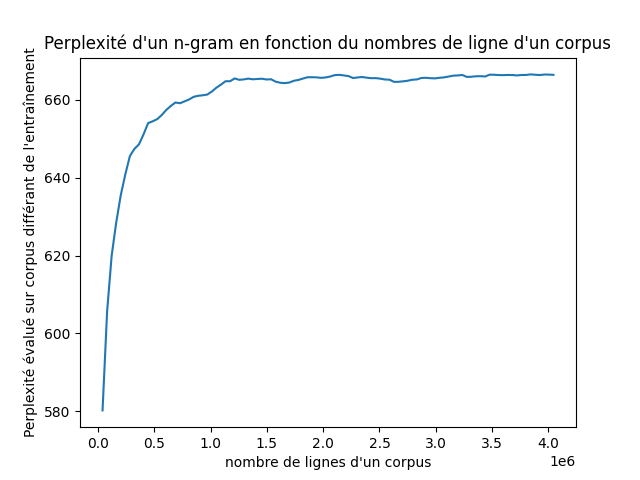
\includegraphics[width=\textwidth]{../results/balzac_result/balzac_1_lines.png}
      \caption{Perplexité d'un unigram en fonction du nombre de ligne}
    \end{subfigure}
    \hfill
    \begin{subfigure}{0.47\textwidth}
      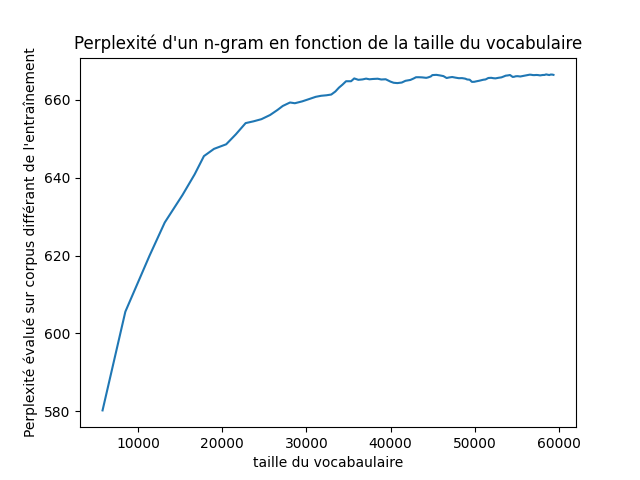
\includegraphics[width=\linewidth]{../results/balzac_result/balzac_1_vocab_size.png}
      \caption{Perplexité d'un unigram en fonction de la taille du vocabulaire}
    \end{subfigure}

    \begin{subfigure}{0.47\textwidth}
        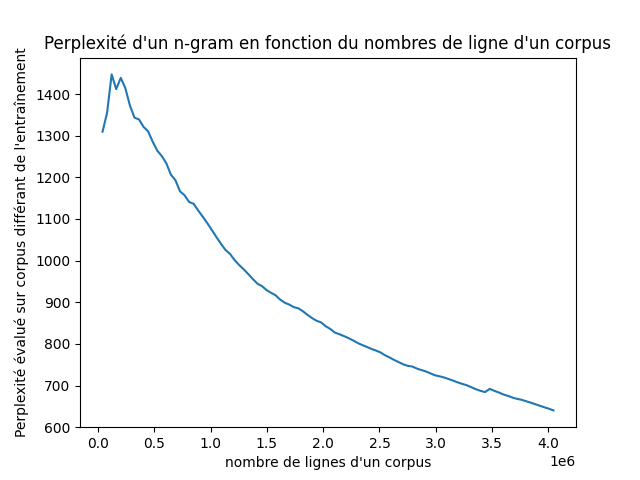
\includegraphics[width=\linewidth]{../results/balzac_result/balzac_2_lines.png}
        \caption{Perplexité d'un bigram en fonction du nombre de ligne}
      \end{subfigure}
      \hfill
      \begin{subfigure}{0.47\textwidth}
        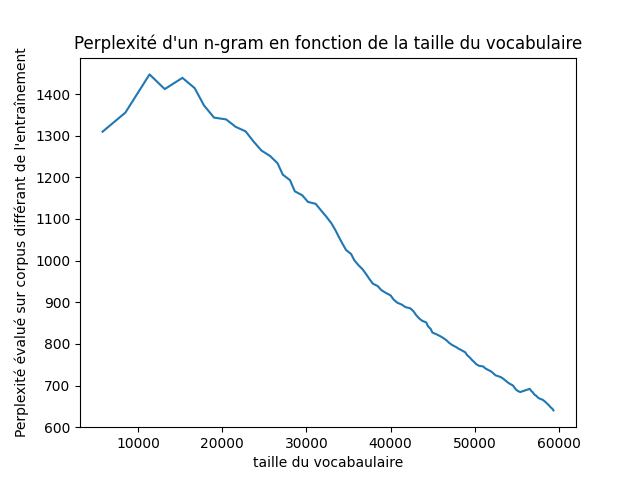
\includegraphics[width=\linewidth]{../results/balzac_result/balzac_2_vocab_size.png}
        \caption{Perplexité d'un bigram en fonction de la taille du vocabulaire}
      \end{subfigure}

      \begin{subfigure}{0.47\textwidth}
        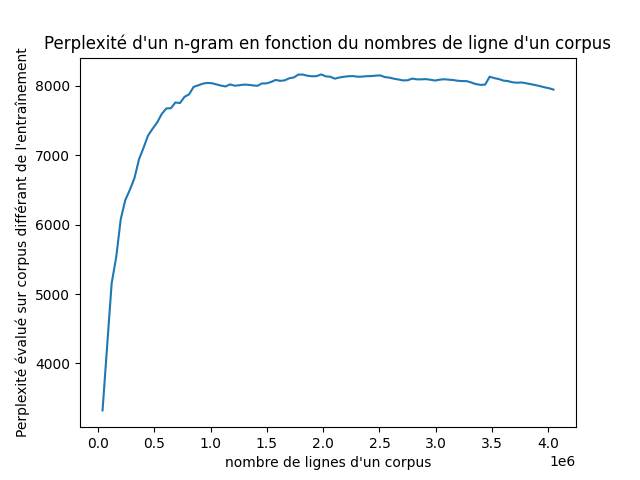
\includegraphics[width=\linewidth]{../results/balzac_result/balzac_3_lines.png}
        \caption{Perplexité d'un trigram en fonction du nombre de ligne}
      \end{subfigure}
      \hfill
      \begin{subfigure}{0.47\textwidth}
        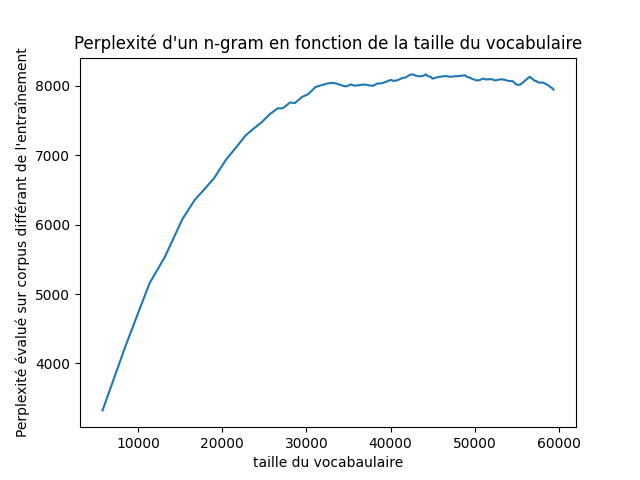
\includegraphics[width=\linewidth]{../results/balzac_result/balzac_3_vocab_size.png}
        \caption{Perplexité d'un trigram en fonction de la taille du vocabulaire}
      \end{subfigure}
      \caption{Perplexité des n-gram en fonction de la taille d'un corpus (à gauche) et de la taille du vocabulaire (à droite).}
      \label{fig: balzac results}
\end{figure}


\section{Piste à creuser 2 : Paternité}

\subsection{Description}
Nous pouvons nous servir d'un modèle de langage pour identifier l'auteur d'un texte. Pour cela, nous l'avons appliqué dans la paternité d'un artiste à ses paroles de chansons. 

\subsection{Mise en oeuvre}
Pour cela, nous avons récolté les fichiers textes de chansons de 10 artistes francophones à l'aide de l'API de Genius. Les 
fichiers ont été pré-traités et mis en forme puis tokenisés par nos soins à l'aide des fichiers de pré-traitement. 

Puis nous entraînons un modèle pour chaque artiste considéré. Chaque modèle effectuera une inférence pour un fichier de paroles test 
désigné, et celui avec la plus petite perplexité correspondra alors au modèle (correspondant à un artiste) qui représente au mieux les 
paroles considérées. On retrouve alors la paternité des paroles de chansons considérées. 

\subsection{Résultats}

Dans un premier temps, il est intéressant d'observer la taille du vocabulaire utilisé par les artistes en question. Cela est montré
par la Figure~\ref{fig:vocab_size}.

\begin{figure}[!ht]
    \centering
    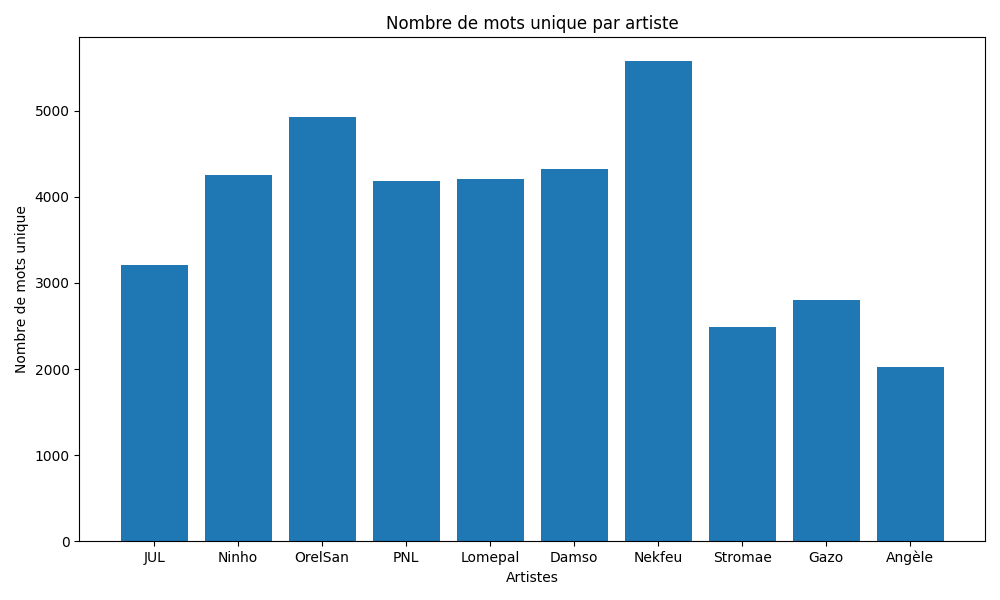
\includegraphics[width=0.7\linewidth]{../results/genius_results/vocab_size_per_artist.png}
    \caption{Taille du vocabulaire de l'ensemble des paroles des chansons selon les artistes}
    \label{fig:vocab_size}
\end{figure}

Ensuite, nous avons entraîné un modèle pour chaque artiste et nous avons comparé la perplexité entre tous les
modèles et tous les textes de test de chaque artiste. On imagine que sur un texte d'un artiste le modèle le plus
performant sera le modèle de l'artiste en question. Grâce à ce procédé, on pourrait retrouver le chanteur si l'on connaît
les paroles d'une chanson. La Figure~\ref{fig:Angele} nous montre les résultats des perplexités des modèles sur un texte d'Angèle.

\begin{figure}[!ht]
    \begin{subfigure}{0.32\textwidth}
        \centering
        \includegraphics[width=\linewidth]{../results/genius_results/Angèle_1.png}
        \caption{modèles unigrams}
    \end{subfigure}
    \hfill
    \begin{subfigure}{0.32\textwidth}
        \centering
        \includegraphics[width=\linewidth]{../results/genius_results/Angèle_2.png}
        \caption{modèles bigrams}
    \end{subfigure}
    \hfill
    \begin{subfigure}{0.32\textwidth}
        \centering
        \includegraphics[width=\linewidth]{../results/genius_results/Angèle_3.png}
        \caption{modèles trigrams}
    \end{subfigure}
    \hfill
    \caption{Préplexités des modèles sur un texte d'Angèle.}
    \label{fig:Angele}
\end{figure}

On peut voir qu'on a bien le modèle d'Angèle qui est le meilleur parmi les modèles de langues apprises sur les paroles d'autres chanteurs.
Cependant, comme on peut le voir dans la Figure~\ref{fig:paternite}, ce n'est pas toujours le cas.


\begin{figure}[!ht]
    \begin{subfigure}{0.32\textwidth}
        \centering
        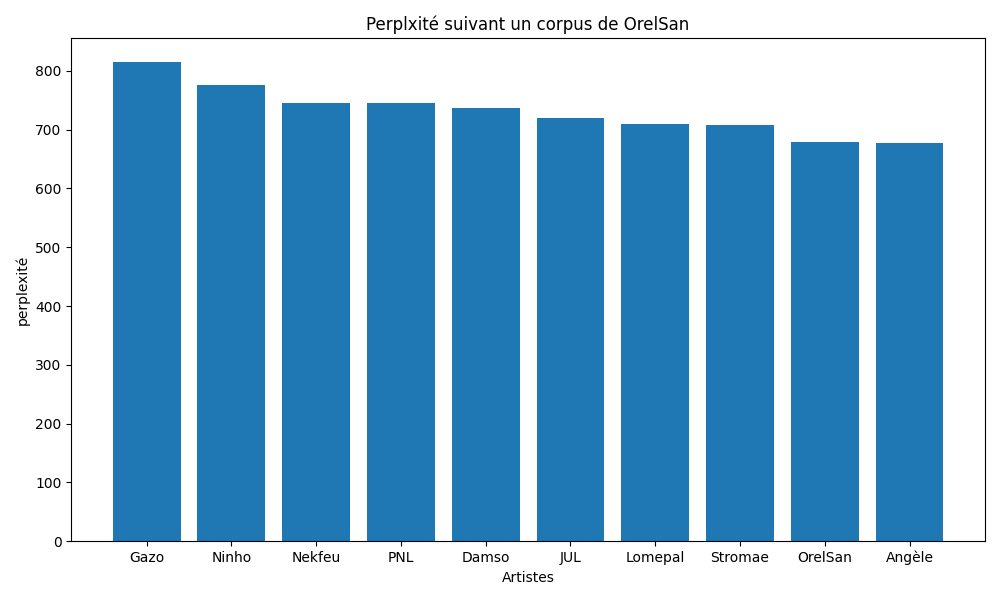
\includegraphics[width=\linewidth]{../results/genius_results/OrelSan_1.png}
        \caption{modèles unigrams sur un texte de OrelSan}
    \end{subfigure}
    \hfill
    \begin{subfigure}{0.32\textwidth}
        \centering
        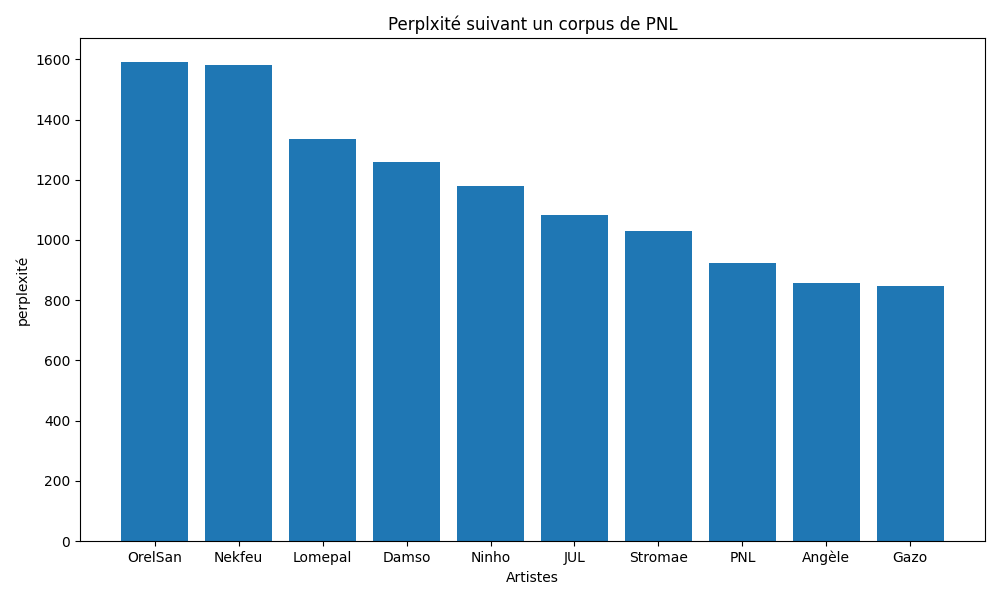
\includegraphics[width=\linewidth]{../results/genius_results/PNL_2.png}
        \caption{modèles bigrams sur un texte de PNL}
    \end{subfigure}
    \hfill
    \begin{subfigure}{0.32\textwidth}
        \centering
        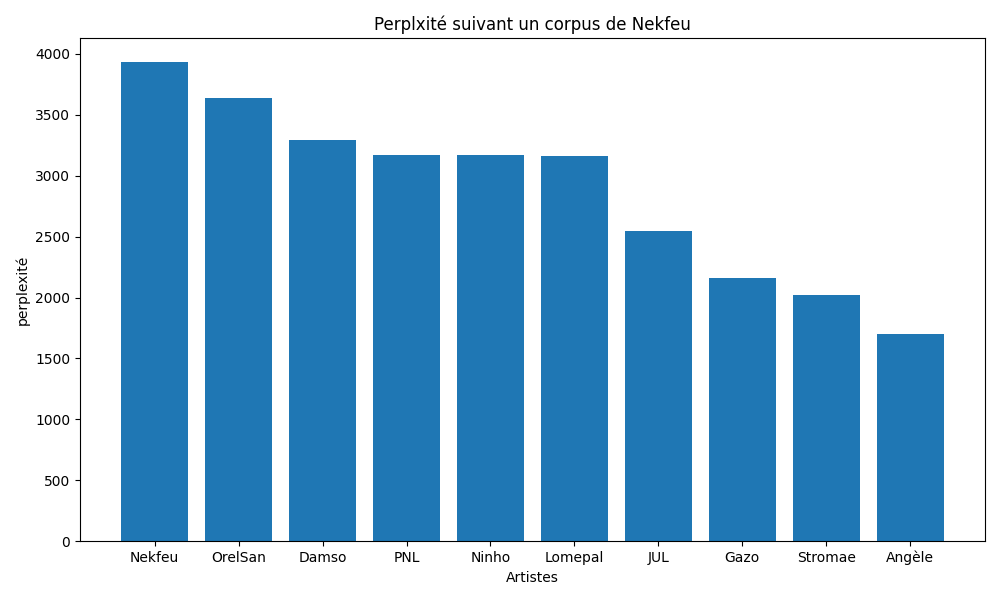
\includegraphics[width=\linewidth]{../results/genius_results/Nekfeu_3.png}
        \caption{modèles trigrams sur un texte de Nekfeu}
    \end{subfigure}
    \hfill
    \caption{Perplexités des modèles où le modèle de l'artiste n'est pas le meilleur.}
    \label{fig:paternite}
\end{figure}

Dans les faits, cela arrive assez souvent. Sur les 10 artistes que l'on a testé, on trouve que les modèles
unigram ont trouvé le bon artiste 8 fois tandis que les bigrams et trigrams l'ont trouvé seulement 2 fois (pour Angèle et Gazo).
Cela peut facilement s'expliquer car les artistes ont parfois des mots qui leurs sont propres (comme 
les noms de leurs labels au début dans le rap français). Mais on observe aussi ceux qui ont une perplexité faible
par rapport aux autres sont pratiquement toujours Angèle, Gazo et Stromae, c'est à dire ce qu'ils ont la taille de 
vocabulaire la plus petite et inversement (voir Figure~\ref{fig:vocab_size}). Cela n'est pas anodin, car 
lorsqu'on calcule la perplexité, le terme $P(m_i|m_{i-n+1},\dots,m_{i-1})$ est divisé par le nombre de mot plus la taille du 
vocabulaire (voir les formules de la Table~\ref{tab:ngram}). Cette quantité est donc généralement plus grande et donc avoir une meilleure perplexité.

On a ensuite voulu aller encore plus loin, en essayant de projeter les artistes dans un espace de dimension 2 et de les représenter de tel
sorte à ce que plus les artistes soit éloignés, plus leurs vocabulaires sont lointains. Pour se faire, on note $(a_i)_{i \in [1, 10]}$ les artistes,
et $PP_{a_i}^{(n)}(T_{a_j})$ la perplexité du n-gram appris sur les textes de l'artiste $i$ évalué sur un texte de l'artiste $j$.
On définit alors une matrice de distance $D^{(n)} \in \mathcal{M}_{10, 10}(\mathbb{R^+})$ qui vérifie l'équation~\ref{eq:def distance}. Cette matrice
est bien symétrique par construction, et on a l'équivalence: plus 2 artistes $i$ et $j$ sont proches, plus $D_{i,j}^{(n)}$ est petit.

\begin{equation}
    D_{i,j}^{(n)} =
    \begin{cases}
    \frac{1}{2}(PP_{a_i}^{(n)}(T_{a_j}) + PP_{a_j}^{(n)}(T_{a_i}))& \text{si } i \neq j \\
    0 & \text{si } i = j
    \end{cases}
    \label{eq:def distance}
\end{equation}

Une fois qu'on a cette matrice de distance, on peut appliquer le Multidimensional scaling (MDS) pour réduire la dimension de l'espace.
En appliquant la MDS pour $n \in \{1, 2, 3\}$, on obtient la Figure~\ref{fig:MDS}. On remarque qu'il n'y a pas de "clusters" formés entre les artistes analysés. Les artistes se différencient bien entre eux par leurs paroles de chansons. 

\begin{figure}[ht]
    \begin{subfigure}{0.32\textwidth}
        \centering
        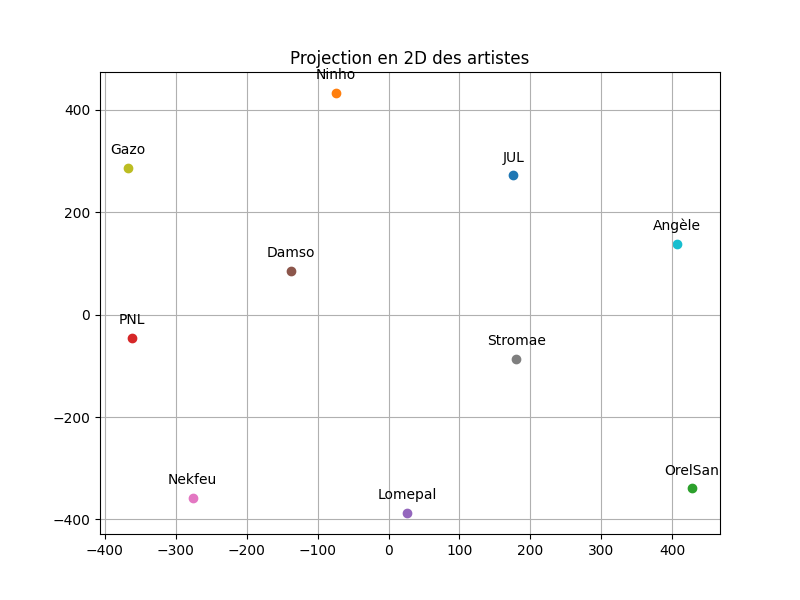
\includegraphics[width=\linewidth]{../results/genius_results/MDS_1.png}
        \caption{unigram}
    \end{subfigure}
    \hfill
    \begin{subfigure}{0.32\textwidth}
        \centering
        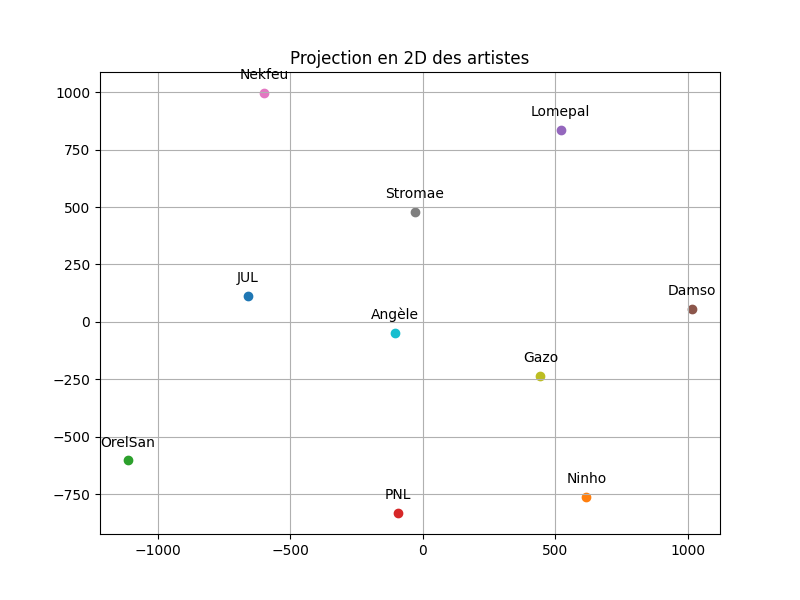
\includegraphics[width=\linewidth]{../results/genius_results/MDS_2.png}
        \caption{bigram}
    \end{subfigure}
    \hfill
    \begin{subfigure}{0.32\textwidth}
        \centering
        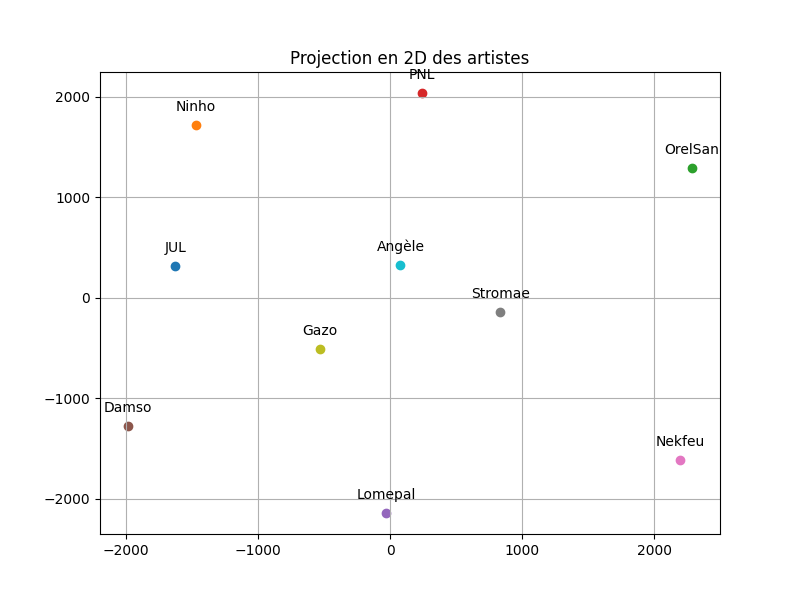
\includegraphics[width=\linewidth]{../results/genius_results/MDS_3.png}
        \caption{trigram}
    \end{subfigure}
    \hfill
    \caption{Projection des artistes dans un espace à 2 dimension avec l'algorithme MDS.}
    \label{fig:MDS}
\end{figure}



\section{Conclusions et perspectives}
Les modèles de langage markoviens soulignent l'importance de prendre en compte le contexte global textuel pour une meilleure 
performance dans le traitement du langage. En effet, les modèles unigrams sont peu voire pas performants, car considérer mot par 
mot un texte va à l'encontre de la compréhension d'un texte dans son ensemble. De plus, considérer le contexte local assez réduit 
du corpus analysé ne permet pas au modèle de comprendre la syntaxe linguistique, d'où l'apparition d'une même séquence que cela soit 
dans le remplissage de texte à trou ou dans la génération de texte. Les modèles bigrams et trigrams sont peu performants également, 
cependant, ils permettent de voir que la prise en compte du contexte permet de noter une relative amélioration par rapport au modèle 
unigram, bien qu'ils ne prennent en compte que quelques séquences de mots précédant la séquence considérée, ce qui reste peu suffisant 
pour généraliser un traitement du langage. 

Les modèles de langages markoviens posent les bases de ce que signifie le traitement du langage, en reproduisant la lecture 
unidirectionnelle du texte par exemple. Malgré tout, les modèles markoviens ne sont pas suffisants en terme de performances pour 
prendre en compte un texte dans sa globalité, notamment en terme de linguistique, de signification et de contexte global, sans 
parler de la prise en compte d'une mémoire long terme afin de créer une connaissance du contexte plus global et général du corpus 
traité. 

\end{document}